% Created by tikzDevice version 0.12.3 on 2019-08-15 12:03:01
% !TEX encoding = UTF-8 Unicode
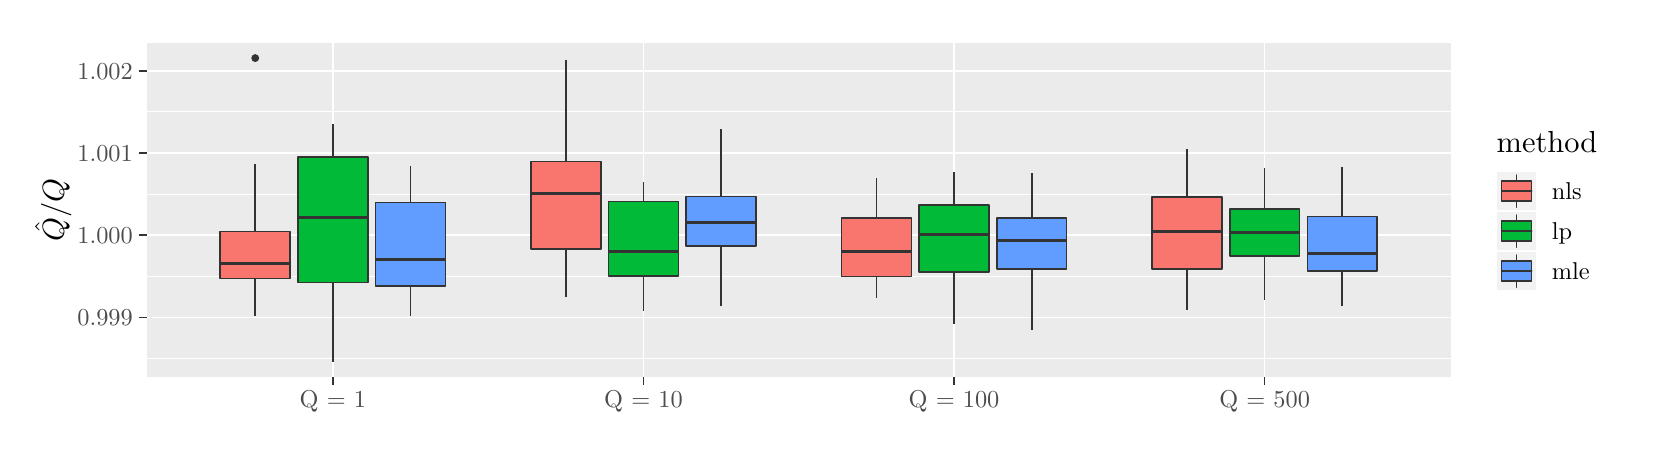
\begin{tikzpicture}[x=1pt,y=1pt]
\definecolor{fillColor}{RGB}{255,255,255}
\path[use as bounding box,fill=fillColor,fill opacity=0.00] (0,0) rectangle (578.16,144.54);
\begin{scope}
\path[clip] (  0.00,  0.00) rectangle (578.16,144.54);
\definecolor{drawColor}{RGB}{255,255,255}
\definecolor{fillColor}{RGB}{255,255,255}

\path[draw=drawColor,line width= 0.6pt,line join=round,line cap=round,fill=fillColor] (  0.00,  0.00) rectangle (578.16,144.54);
\end{scope}
\begin{scope}
\path[clip] ( 42.95, 18.22) rectangle (514.31,139.04);
\definecolor{fillColor}{gray}{0.92}

\path[fill=fillColor] ( 42.95, 18.22) rectangle (514.31,139.04);
\definecolor{drawColor}{RGB}{255,255,255}

\path[draw=drawColor,line width= 0.3pt,line join=round] ( 42.95, 24.94) --
	(514.31, 24.94);

\path[draw=drawColor,line width= 0.3pt,line join=round] ( 42.95, 54.67) --
	(514.31, 54.67);

\path[draw=drawColor,line width= 0.3pt,line join=round] ( 42.95, 84.41) --
	(514.31, 84.41);

\path[draw=drawColor,line width= 0.3pt,line join=round] ( 42.95,114.14) --
	(514.31,114.14);

\path[draw=drawColor,line width= 0.6pt,line join=round] ( 42.95, 39.81) --
	(514.31, 39.81);

\path[draw=drawColor,line width= 0.6pt,line join=round] ( 42.95, 69.54) --
	(514.31, 69.54);

\path[draw=drawColor,line width= 0.6pt,line join=round] ( 42.95, 99.27) --
	(514.31, 99.27);

\path[draw=drawColor,line width= 0.6pt,line join=round] ( 42.95,129.00) --
	(514.31,129.00);

\path[draw=drawColor,line width= 0.6pt,line join=round] (110.29, 18.22) --
	(110.29,139.04);

\path[draw=drawColor,line width= 0.6pt,line join=round] (222.52, 18.22) --
	(222.52,139.04);

\path[draw=drawColor,line width= 0.6pt,line join=round] (334.74, 18.22) --
	(334.74,139.04);

\path[draw=drawColor,line width= 0.6pt,line join=round] (446.97, 18.22) --
	(446.97,139.04);
\definecolor{drawColor}{gray}{0.20}
\definecolor{fillColor}{gray}{0.20}

\path[draw=drawColor,line width= 0.4pt,line join=round,line cap=round,fill=fillColor] ( 82.23,133.55) circle (  1.21);

\path[draw=drawColor,line width= 0.6pt,line join=round] ( 82.23, 70.86) -- ( 82.23, 95.15);

\path[draw=drawColor,line width= 0.6pt,line join=round] ( 82.23, 53.89) -- ( 82.23, 40.42);
\definecolor{fillColor}{RGB}{248,118,109}

\path[draw=drawColor,line width= 0.6pt,line join=round,line cap=round,fill=fillColor] ( 69.61, 70.86) --
	( 69.61, 53.89) --
	( 94.86, 53.89) --
	( 94.86, 70.86) --
	( 69.61, 70.86) --
	cycle;

\path[draw=drawColor,line width= 1.1pt,line join=round] ( 69.61, 59.35) -- ( 94.86, 59.35);

\path[draw=drawColor,line width= 0.6pt,line join=round] (110.29, 97.82) -- (110.29,109.88);

\path[draw=drawColor,line width= 0.6pt,line join=round] (110.29, 52.48) -- (110.29, 23.71);
\definecolor{fillColor}{RGB}{0,186,56}

\path[draw=drawColor,line width= 0.6pt,line join=round,line cap=round,fill=fillColor] ( 97.66, 97.82) --
	( 97.66, 52.48) --
	(122.92, 52.48) --
	(122.92, 97.82) --
	( 97.66, 97.82) --
	cycle;

\path[draw=drawColor,line width= 1.1pt,line join=round] ( 97.66, 75.83) -- (122.92, 75.83);

\path[draw=drawColor,line width= 0.6pt,line join=round] (138.35, 81.33) -- (138.35, 94.57);

\path[draw=drawColor,line width= 0.6pt,line join=round] (138.35, 51.17) -- (138.35, 40.33);
\definecolor{fillColor}{RGB}{97,156,255}

\path[draw=drawColor,line width= 0.6pt,line join=round,line cap=round,fill=fillColor] (125.72, 81.33) --
	(125.72, 51.17) --
	(150.97, 51.17) --
	(150.97, 81.33) --
	(125.72, 81.33) --
	cycle;

\path[draw=drawColor,line width= 1.1pt,line join=round] (125.72, 60.86) -- (150.97, 60.86);

\path[draw=drawColor,line width= 0.6pt,line join=round] (194.46, 96.19) -- (194.46,132.80);

\path[draw=drawColor,line width= 0.6pt,line join=round] (194.46, 64.67) -- (194.46, 47.37);
\definecolor{fillColor}{RGB}{248,118,109}

\path[draw=drawColor,line width= 0.6pt,line join=round,line cap=round,fill=fillColor] (181.83, 96.19) --
	(181.83, 64.67) --
	(207.09, 64.67) --
	(207.09, 96.19) --
	(181.83, 96.19) --
	cycle;

\path[draw=drawColor,line width= 1.1pt,line join=round] (181.83, 84.67) -- (207.09, 84.67);

\path[draw=drawColor,line width= 0.6pt,line join=round] (222.52, 81.74) -- (222.52, 88.81);

\path[draw=drawColor,line width= 0.6pt,line join=round] (222.52, 54.71) -- (222.52, 42.22);
\definecolor{fillColor}{RGB}{0,186,56}

\path[draw=drawColor,line width= 0.6pt,line join=round,line cap=round,fill=fillColor] (209.89, 81.74) --
	(209.89, 54.71) --
	(235.14, 54.71) --
	(235.14, 81.74) --
	(209.89, 81.74) --
	cycle;

\path[draw=drawColor,line width= 1.1pt,line join=round] (209.89, 63.58) -- (235.14, 63.58);

\path[draw=drawColor,line width= 0.6pt,line join=round] (250.57, 83.54) -- (250.57,108.10);

\path[draw=drawColor,line width= 0.6pt,line join=round] (250.57, 65.65) -- (250.57, 44.11);
\definecolor{fillColor}{RGB}{97,156,255}

\path[draw=drawColor,line width= 0.6pt,line join=round,line cap=round,fill=fillColor] (237.95, 83.54) --
	(237.95, 65.65) --
	(263.20, 65.65) --
	(263.20, 83.54) --
	(237.95, 83.54) --
	cycle;

\path[draw=drawColor,line width= 1.1pt,line join=round] (237.95, 74.27) -- (263.20, 74.27);

\path[draw=drawColor,line width= 0.6pt,line join=round] (306.69, 75.84) -- (306.69, 90.07);

\path[draw=drawColor,line width= 0.6pt,line join=round] (306.69, 54.59) -- (306.69, 46.76);
\definecolor{fillColor}{RGB}{248,118,109}

\path[draw=drawColor,line width= 0.6pt,line join=round,line cap=round,fill=fillColor] (294.06, 75.84) --
	(294.06, 54.59) --
	(319.31, 54.59) --
	(319.31, 75.84) --
	(294.06, 75.84) --
	cycle;

\path[draw=drawColor,line width= 1.1pt,line join=round] (294.06, 63.80) -- (319.31, 63.80);

\path[draw=drawColor,line width= 0.6pt,line join=round] (334.74, 80.45) -- (334.74, 92.55);

\path[draw=drawColor,line width= 0.6pt,line join=round] (334.74, 56.27) -- (334.74, 37.29);
\definecolor{fillColor}{RGB}{0,186,56}

\path[draw=drawColor,line width= 0.6pt,line join=round,line cap=round,fill=fillColor] (322.12, 80.45) --
	(322.12, 56.27) --
	(347.37, 56.27) --
	(347.37, 80.45) --
	(322.12, 80.45) --
	cycle;

\path[draw=drawColor,line width= 1.1pt,line join=round] (322.12, 69.77) -- (347.37, 69.77);

\path[draw=drawColor,line width= 0.6pt,line join=round] (362.80, 75.72) -- (362.80, 92.18);

\path[draw=drawColor,line width= 0.6pt,line join=round] (362.80, 57.42) -- (362.80, 35.45);
\definecolor{fillColor}{RGB}{97,156,255}

\path[draw=drawColor,line width= 0.6pt,line join=round,line cap=round,fill=fillColor] (350.18, 75.72) --
	(350.18, 57.42) --
	(375.43, 57.42) --
	(375.43, 75.72) --
	(350.18, 75.72) --
	cycle;

\path[draw=drawColor,line width= 1.1pt,line join=round] (350.18, 67.77) -- (375.43, 67.77);

\path[draw=drawColor,line width= 0.6pt,line join=round] (418.91, 83.44) -- (418.91,100.72);

\path[draw=drawColor,line width= 0.6pt,line join=round] (418.91, 57.39) -- (418.91, 42.68);
\definecolor{fillColor}{RGB}{248,118,109}

\path[draw=drawColor,line width= 0.6pt,line join=round,line cap=round,fill=fillColor] (406.29, 83.44) --
	(406.29, 57.39) --
	(431.54, 57.39) --
	(431.54, 83.44) --
	(406.29, 83.44) --
	cycle;

\path[draw=drawColor,line width= 1.1pt,line join=round] (406.29, 70.87) -- (431.54, 70.87);

\path[draw=drawColor,line width= 0.6pt,line join=round] (446.97, 78.90) -- (446.97, 93.74);

\path[draw=drawColor,line width= 0.6pt,line join=round] (446.97, 62.13) -- (446.97, 46.04);
\definecolor{fillColor}{RGB}{0,186,56}

\path[draw=drawColor,line width= 0.6pt,line join=round,line cap=round,fill=fillColor] (434.35, 78.90) --
	(434.35, 62.13) --
	(459.60, 62.13) --
	(459.60, 78.90) --
	(434.35, 78.90) --
	cycle;

\path[draw=drawColor,line width= 1.1pt,line join=round] (434.35, 70.52) -- (459.60, 70.52);

\path[draw=drawColor,line width= 0.6pt,line join=round] (475.03, 76.35) -- (475.03, 94.25);

\path[draw=drawColor,line width= 0.6pt,line join=round] (475.03, 56.60) -- (475.03, 43.95);
\definecolor{fillColor}{RGB}{97,156,255}

\path[draw=drawColor,line width= 0.6pt,line join=round,line cap=round,fill=fillColor] (462.40, 76.35) --
	(462.40, 56.60) --
	(487.65, 56.60) --
	(487.65, 76.35) --
	(462.40, 76.35) --
	cycle;

\path[draw=drawColor,line width= 1.1pt,line join=round] (462.40, 63.01) -- (487.65, 63.01);
\end{scope}
\begin{scope}
\path[clip] (  0.00,  0.00) rectangle (578.16,144.54);
\definecolor{drawColor}{gray}{0.30}

\node[text=drawColor,anchor=base east,inner sep=0pt, outer sep=0pt, scale=  0.88] at ( 38.00, 36.78) {0.999};

\node[text=drawColor,anchor=base east,inner sep=0pt, outer sep=0pt, scale=  0.88] at ( 38.00, 66.51) {1.000};

\node[text=drawColor,anchor=base east,inner sep=0pt, outer sep=0pt, scale=  0.88] at ( 38.00, 96.24) {1.001};

\node[text=drawColor,anchor=base east,inner sep=0pt, outer sep=0pt, scale=  0.88] at ( 38.00,125.97) {1.002};
\end{scope}
\begin{scope}
\path[clip] (  0.00,  0.00) rectangle (578.16,144.54);
\definecolor{drawColor}{gray}{0.20}

\path[draw=drawColor,line width= 0.6pt,line join=round] ( 40.20, 39.81) --
	( 42.95, 39.81);

\path[draw=drawColor,line width= 0.6pt,line join=round] ( 40.20, 69.54) --
	( 42.95, 69.54);

\path[draw=drawColor,line width= 0.6pt,line join=round] ( 40.20, 99.27) --
	( 42.95, 99.27);

\path[draw=drawColor,line width= 0.6pt,line join=round] ( 40.20,129.00) --
	( 42.95,129.00);
\end{scope}
\begin{scope}
\path[clip] (  0.00,  0.00) rectangle (578.16,144.54);
\definecolor{drawColor}{gray}{0.20}

\path[draw=drawColor,line width= 0.6pt,line join=round] (110.29, 15.47) --
	(110.29, 18.22);

\path[draw=drawColor,line width= 0.6pt,line join=round] (222.52, 15.47) --
	(222.52, 18.22);

\path[draw=drawColor,line width= 0.6pt,line join=round] (334.74, 15.47) --
	(334.74, 18.22);

\path[draw=drawColor,line width= 0.6pt,line join=round] (446.97, 15.47) --
	(446.97, 18.22);
\end{scope}
\begin{scope}
\path[clip] (  0.00,  0.00) rectangle (578.16,144.54);
\definecolor{drawColor}{gray}{0.30}

\node[text=drawColor,anchor=base,inner sep=0pt, outer sep=0pt, scale=  0.88] at (110.29,  7.21) {Q = 1};

\node[text=drawColor,anchor=base,inner sep=0pt, outer sep=0pt, scale=  0.88] at (222.52,  7.21) {Q = 10};

\node[text=drawColor,anchor=base,inner sep=0pt, outer sep=0pt, scale=  0.88] at (334.74,  7.21) {Q = 100};

\node[text=drawColor,anchor=base,inner sep=0pt, outer sep=0pt, scale=  0.88] at (446.97,  7.21) {Q = 500};
\end{scope}
\begin{scope}
\path[clip] (  0.00,  0.00) rectangle (578.16,144.54);
\definecolor{drawColor}{RGB}{0,0,0}

\node[text=drawColor,rotate= 90.00,anchor=base,inner sep=0pt, outer sep=0pt, scale=  1.10] at ( 13.08, 78.63) {$\hat{Q}/Q$};
\end{scope}
\begin{scope}
\path[clip] (  0.00,  0.00) rectangle (578.16,144.54);
\definecolor{fillColor}{RGB}{255,255,255}

\path[fill=fillColor] (525.31, 43.84) rectangle (572.66,113.42);
\end{scope}
\begin{scope}
\path[clip] (  0.00,  0.00) rectangle (578.16,144.54);
\definecolor{drawColor}{RGB}{0,0,0}

\node[text=drawColor,anchor=base west,inner sep=0pt, outer sep=0pt, scale=  1.10] at (530.81, 99.27) {method};
\end{scope}
\begin{scope}
\path[clip] (  0.00,  0.00) rectangle (578.16,144.54);
\definecolor{drawColor}{RGB}{255,255,255}
\definecolor{fillColor}{gray}{0.95}

\path[draw=drawColor,line width= 0.6pt,line join=round,line cap=round,fill=fillColor] (530.81, 78.25) rectangle (545.26, 92.70);
\end{scope}
\begin{scope}
\path[clip] (  0.00,  0.00) rectangle (578.16,144.54);
\definecolor{drawColor}{gray}{0.20}

\path[draw=drawColor,line width= 0.6pt,line join=round,line cap=round] (538.03, 79.70) --
	(538.03, 81.86);

\path[draw=drawColor,line width= 0.6pt,line join=round,line cap=round] (538.03, 89.09) --
	(538.03, 91.26);
\definecolor{fillColor}{RGB}{248,118,109}

\path[draw=drawColor,line width= 0.6pt,line join=round,line cap=round,fill=fillColor] (532.61, 81.86) rectangle (543.45, 89.09);

\path[draw=drawColor,line width= 0.6pt,line join=round,line cap=round] (532.61, 85.48) --
	(543.45, 85.48);
\end{scope}
\begin{scope}
\path[clip] (  0.00,  0.00) rectangle (578.16,144.54);
\definecolor{drawColor}{RGB}{255,255,255}
\definecolor{fillColor}{gray}{0.95}

\path[draw=drawColor,line width= 0.6pt,line join=round,line cap=round,fill=fillColor] (530.81, 63.80) rectangle (545.26, 78.25);
\end{scope}
\begin{scope}
\path[clip] (  0.00,  0.00) rectangle (578.16,144.54);
\definecolor{drawColor}{gray}{0.20}

\path[draw=drawColor,line width= 0.6pt,line join=round,line cap=round] (538.03, 65.24) --
	(538.03, 67.41);

\path[draw=drawColor,line width= 0.6pt,line join=round,line cap=round] (538.03, 74.64) --
	(538.03, 76.81);
\definecolor{fillColor}{RGB}{0,186,56}

\path[draw=drawColor,line width= 0.6pt,line join=round,line cap=round,fill=fillColor] (532.61, 67.41) rectangle (543.45, 74.64);

\path[draw=drawColor,line width= 0.6pt,line join=round,line cap=round] (532.61, 71.02) --
	(543.45, 71.02);
\end{scope}
\begin{scope}
\path[clip] (  0.00,  0.00) rectangle (578.16,144.54);
\definecolor{drawColor}{RGB}{255,255,255}
\definecolor{fillColor}{gray}{0.95}

\path[draw=drawColor,line width= 0.6pt,line join=round,line cap=round,fill=fillColor] (530.81, 49.34) rectangle (545.26, 63.80);
\end{scope}
\begin{scope}
\path[clip] (  0.00,  0.00) rectangle (578.16,144.54);
\definecolor{drawColor}{gray}{0.20}

\path[draw=drawColor,line width= 0.6pt,line join=round,line cap=round] (538.03, 50.79) --
	(538.03, 52.96);

\path[draw=drawColor,line width= 0.6pt,line join=round,line cap=round] (538.03, 60.18) --
	(538.03, 62.35);
\definecolor{fillColor}{RGB}{97,156,255}

\path[draw=drawColor,line width= 0.6pt,line join=round,line cap=round,fill=fillColor] (532.61, 52.96) rectangle (543.45, 60.18);

\path[draw=drawColor,line width= 0.6pt,line join=round,line cap=round] (532.61, 56.57) --
	(543.45, 56.57);
\end{scope}
\begin{scope}
\path[clip] (  0.00,  0.00) rectangle (578.16,144.54);
\definecolor{drawColor}{RGB}{0,0,0}

\node[text=drawColor,anchor=base west,inner sep=0pt, outer sep=0pt, scale=  0.88] at (550.76, 82.45) {nls};
\end{scope}
\begin{scope}
\path[clip] (  0.00,  0.00) rectangle (578.16,144.54);
\definecolor{drawColor}{RGB}{0,0,0}

\node[text=drawColor,anchor=base west,inner sep=0pt, outer sep=0pt, scale=  0.88] at (550.76, 67.99) {lp};
\end{scope}
\begin{scope}
\path[clip] (  0.00,  0.00) rectangle (578.16,144.54);
\definecolor{drawColor}{RGB}{0,0,0}

\node[text=drawColor,anchor=base west,inner sep=0pt, outer sep=0pt, scale=  0.88] at (550.76, 53.54) {mle};
\end{scope}
\end{tikzpicture}
